\documentclass[tikz,border=4pt]{standalone}
\usepackage{amsmath,amssymb}
\usetikzlibrary{arrows.meta,calc}
\begin{document}
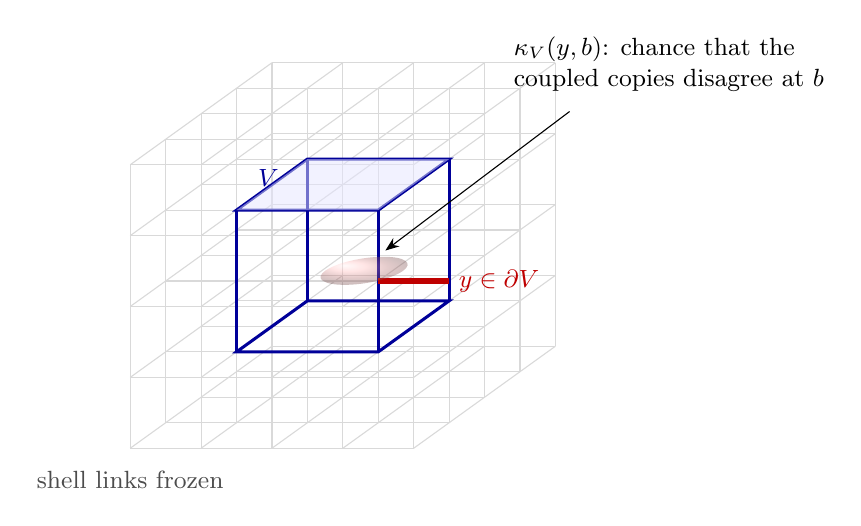
\begin{tikzpicture}[x={(1cm,0cm)},y={(0.5cm,0.36cm)},z={(0cm,1cm)},scale=0.9]
\def\L{4}
% shell (outer cube) light
\foreach \x in {0,...,\L}{\foreach \y in {0,...,\L}{
  \draw[gray!30] (\x,\y,0)--(\x,\y,\L);}}
\foreach \x in {0,...,\L}{\foreach \z in {0,...,\L}{
  \draw[gray!30] (\x,0,\z)--(\x,\L,\z);}}
\foreach \y in {0,...,\L}{\foreach \z in {0,...,\L}{
  \draw[gray!30] (0,\y,\z)--(\L,\y,\z);}}
% inner box
\draw[blue!60!black,line width=1.1pt] (1,1,1)--(3,1,1)--(3,3,1)--(1,3,1)--cycle;
\draw[blue!60!black,line width=1.1pt] (1,1,3)--(3,1,3)--(3,3,3)--(1,3,3)--cycle;
\foreach \a/\b in {1/1,3/1,3/3,1/3}{\draw[blue!60!black,line width=1.1pt] (\a,\b,1)--(\a,\b,3);}
\fill[blue!10,opacity=0.5] (1,1,3)--(3,1,3)--(3,3,3)--(1,3,3)--cycle;
\node[blue!60!black,font=\small] at (1.3,1.3,3.35) {$V$};
% boundary link y
\draw[red!75!black,line width=2.2pt] (3,1,2)--(4,1,2);
\node[red!75!black,right,font=\small] at (4,1,2) {$y\in\partial V$};
% influence cloud
\shade[ball color=red!40,opacity=0.35] (2.6,1.4,2) circle (0.55);
\node[font=\small,align=left] at (5.9,3.4,4.2) {$\kappa_V(y,b)$: chance that the\\ coupled copies disagree at $b$};
\draw[-{Stealth[length=5pt]}] (4.6,3.2,3.6)--(2.85,1.5,2.25);
\node[gray!60!black,font=\small] at (0,0,-0.45) {shell links frozen};
\end{tikzpicture}
\end{document}
